%
% File nodalida2017.tex
%
% Contact beata.megyesi@lingfil.uu.se
%
% Based on the instruction file for Nodalida 2015 and EACL 2014
% which in turn was based on the instruction files for previous 
% ACL and EACL conferences.

\documentclass[11pt]{article}
\usepackage{nodalida2017}
%\usepackage{times}
\usepackage{mathptmx}
%\usepackage{txfonts}
\usepackage{graphicx}
\usepackage{url}
\usepackage{latexsym}
\special{papersize=210mm,297mm} % to avoid having to use "-t a4" with dvips 
%\setlength\titlebox{6.5cm}  % You can expand the title box if you really have to

\title{Exploring the Expressivity of Constraint Grammar}

% \author{First Author \\
%   Affiliation / Address line 1 \\
%   Affiliation / Address line 2 \\
%   Affiliation / Address line 3 \\
%   {\tt email@domain} \\\And
%   Second Author \\
%   Affiliation / Address line 1 \\
%   Affiliation / Address line 2 \\
%   Affiliation / Address line 3 \\
%   {\tt email@domain} \\}

\date{}

\def\t#1{\texttt{#1}}

\begin{document}
\maketitle

% \begin{abstract}
%   This document contains the instructions for preparing a camera-ready
%   manuscript for the proceedings of Nodalida-2017. The document itself
%   conforms to its own specifications, and is therefore an example of
%   what your manuscript should look like. These instructions should be
%   used for both papers submitted for review and for final versions of
%   accepted papers.  Authors are asked to conform to all the directions
%   reported in this document.
% \end{abstract}


\section{Introduction}

Traditionally, CG is seen as a practical and language-oriented approach to NLP; it is a tool rather than a formalism, framework or anything of the sort. Since the beginning of CG \cite{karlsson1995constraint}, its authors do not envision CG being capable of generation, only for analysis. Despite its decidedly linguistic roots, we argue that CG is interesting to look at also from a computational perspective. For the theoretically inclined, making a description of a formalism more precise is an end of its own. However, even a practically oriented reader should appreciate the applications: better understanding of a formalism may lead to novel uses and implementation techniques. In this paper, we address the question of the expressivity of CG. We do not reach a definite answer, but hope to create new ways to reason about reductionistic grammar formalisms.

\section{Background and previous work}


The standard measure of formal languages is the Chomsky hierarchy~\cite{chomsky1956hierarchy}, with its four
classes of grammars and languages, in order from most expressive to least expressive:
recursively enumerable (Type 0), context-sensitive (Type 1), context-free (Type 2), and
regular (Type 3).
The notion of expressive power, ``which constructs can we express in the language'', is coupled with parsing complexity, ``how much time and memory do we need to parse sentences in the language''; more expressive power corresponds to greater parsing complexity.

Previous work covers the expressivity of single rules, such as \texttt{IF (NOT 1* Verb OR Noun)}: just seeing this contextual test hints that we can express a subset of regular languages that contains at least disjunction, complement and Kleene star. 
\newcite{tapanainen1999phd} gives a precise definition of the expressivity of a single rule for 4 different constraint formalisms. In addition, parsing complexity can be easily defined for a given variant and implementation of CG; see for instance \newcite{nemeskey14}.

However, the expressivity of the whole grammar is harder to define. 
A given grammar in CG does not describe a language, but a \emph{relation} between an input language and an output language. 
In the following section, we introduce our approach to emulating generation, and in the rest of the paper, we present some preliminary results.

\section{Expressivity of a grammar}

We view a constraint grammar as a formal language $\mathcal{L}$, generated over an 
alphabet $\Sigma$. We generate the strings in our language by passing 
\emph{maximally ambiguous strings} of every length to the grammar. 
With maximally ambiguous, we mean those strings where each cohort contains the 
entire alphabet, written as $\langle \Sigma \rangle_n$. 
A constraint grammar is said to accept a string $w$ of length $n$ if, 
when we pass $\langle \Sigma \rangle_n$ as an input to the CG,
$w$ is one of the possible interpretations of its output.

For example, consider the language $a*$ over $\Sigma = \{a,b\}$,
shown in Figure~\ref{fig:astar}.
%The initial sentence consists of cohorts with two readings, $a$ and $b$, and the disambiguated sentence has only cohorts with a single reading, $a$. 
The grammar that accepts this language is simply \texttt{SELECT (a)}.

\def\wwf{~~~~\t{"<w>"}}
\def\alm{\t{"a" a}~~~~~~}
\def\blm{\t{"b" b}~~~~~~}

\begin{figure}[h]
\centering

%\begin{tabular}{cl @{\hspace{2cm}} rl}
\begin{tabular}{cl |  rl}
\multicolumn{2}{c|}{\textbf{Input}} & \multicolumn{2}{c}{\textbf{Output}} \\ \hline

\wwf  &        &  \wwf &        \\
         & \alm  &          & \alm  \\
         & \blm  &          &        \\
\wwf  &        &  \wwf &        \\
         & \alm  &          & \alm  \\
         & \blm  &          &        \\
\wwf  &        &  \wwf &        \\
         & \alm  &          & \alm  \\
         & \blm  &          &        \\
\end{tabular}

\caption{Language $a*$ for input $\langle \Sigma \rangle_3$.}
\label{fig:astar}
\end{figure}



\begin{figure}[t]
  \centering
    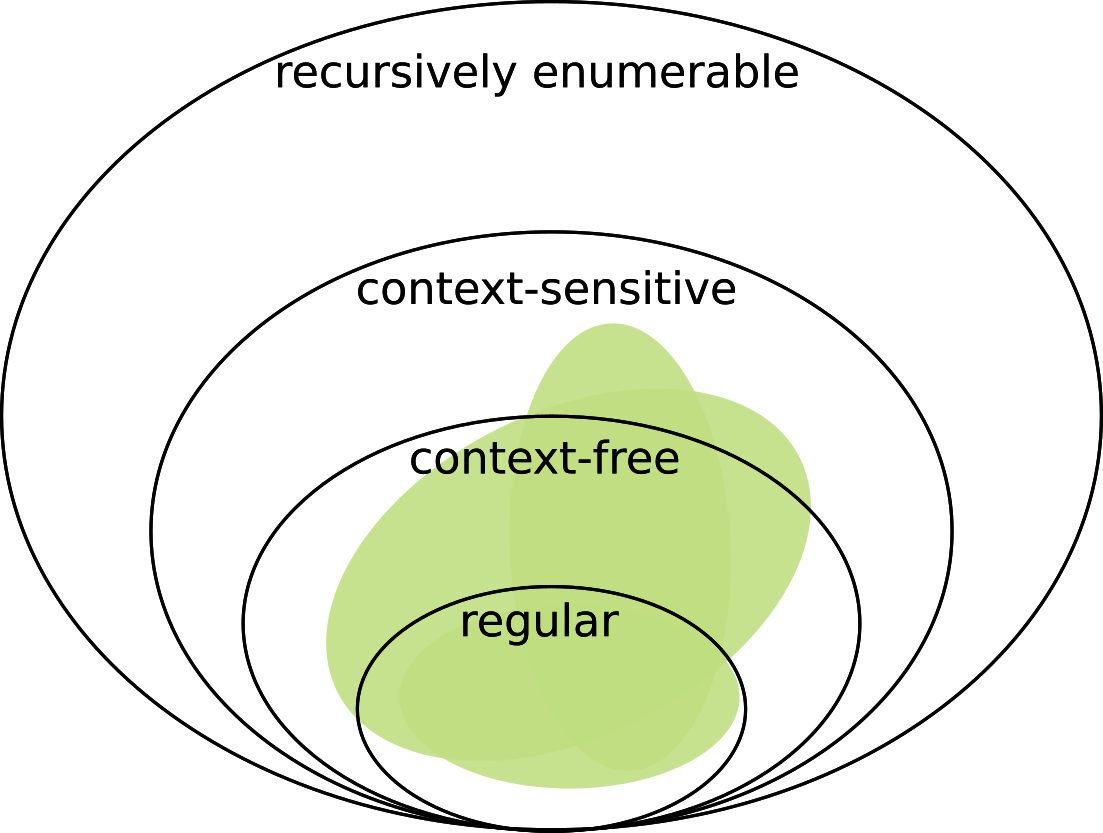
\includegraphics[width=0.4\textwidth]{chomsky.png}
  \caption{A (hypothetical) formalism that does not correspond to any single category in Chomsky hierarchy, but covers some languages in regular, some in context-free and some in context-sensitive class.}
 \label{fig:nocorr}
\end{figure}





We start exploring the expressivity without any previous assumptions. 
For all we know, CG may be in no particular category at all, as shown 
in Figure~\ref{fig:nocorr}. Rather than enumerating individual grammars 
for a given class, we need a method that can transform all languages 
in that class into CG, or prove that there is no such method.

\section{Is CG regular?}

Regular languages can be expressed in the form of finite automata.
For the automaton given in Figure~\ref{fig:fsa}, we implement a corresponding 
CG as follows.

Assume our alphabet is $\Sigma = \{det,adj,noun\}$. Then we have \emph{word cohorts}
$\langle \Sigma \rangle_1$, with \emph{state cohorts} $\langle S \rangle_1$

The transitions are modelled as $\langle \Sigma \rangle_1$ each, but in between each
cohort, we insert a maximally ambiguous \emph{state cohort}, $\langle S \rangle_1$.


For example, a sequence with two transitions would be modelled with the following 
``sentence'' $\langle S+\Sigma \rangle_2$, with two word cohorts, three state cohorts:

\begin{table}[h]
\centering
\begin{tabular}{lllll}
      \t{"<s>"} &  \t{"<w>"}   &      \t{"<s>"} &     \t{"<w>"} &     \t{"<s>"} \\
 ~~~~~~\t{s0}   & ~~~~\t{det}  &  ~~~~\t{ s0}   &  ~~~~\t{det}  &  ~~~~\t{s0}   \\
 ~~~~~~\t{s1}   & ~~~~\t{adj}  &  ~~~~\t{ s1}   &  ~~~~\t{adj}  &  ~~~~\t{s1}    \\
 ~~~~~~\t{s2}   & ~~~~\t{noun} &  ~~~~\t{ s2}   &  ~~~~\t{noun} &  ~~~~\t{s2}  
\end{tabular}
\end{table}

The rules of the grammar disambiguate both word cohorts and state cohorts. 
Given that every transition happens between two states, and every state is 
in between some transition to and from, we can write every rule with exactly
two contextual tests: -1 and 1. 

We begin the disambiguation from the first state cohort, which can only be
the start state. Likewise, the last state cohort may only contain allowed end states.


The start and end states naturally
correspond to the first and last state cohort in the  $\langle S+\Sigma \rangle_n$,
and can be 


% \begin{itemize}
% \item[\t{"<s>"}] ~\\
% 				 \\
% 		      	 \t{"s1" s1 } \\
% 			     \t{"s2" s2 }
% \item [\t{"<w>"}] ~\\
% 				\t{"det" det} \\
% 				\t{"adj" adj} \\
% 				\t{"n"   n}

% \item[\t{"<s>"}] ~\\
% 				 \t{"s0" s0} \\
% 		      	 \t{"s1" s1 } \\
% 			     \t{"s2" s2 }
% \end{itemize}



\begin{figure}[t]
  \centering
    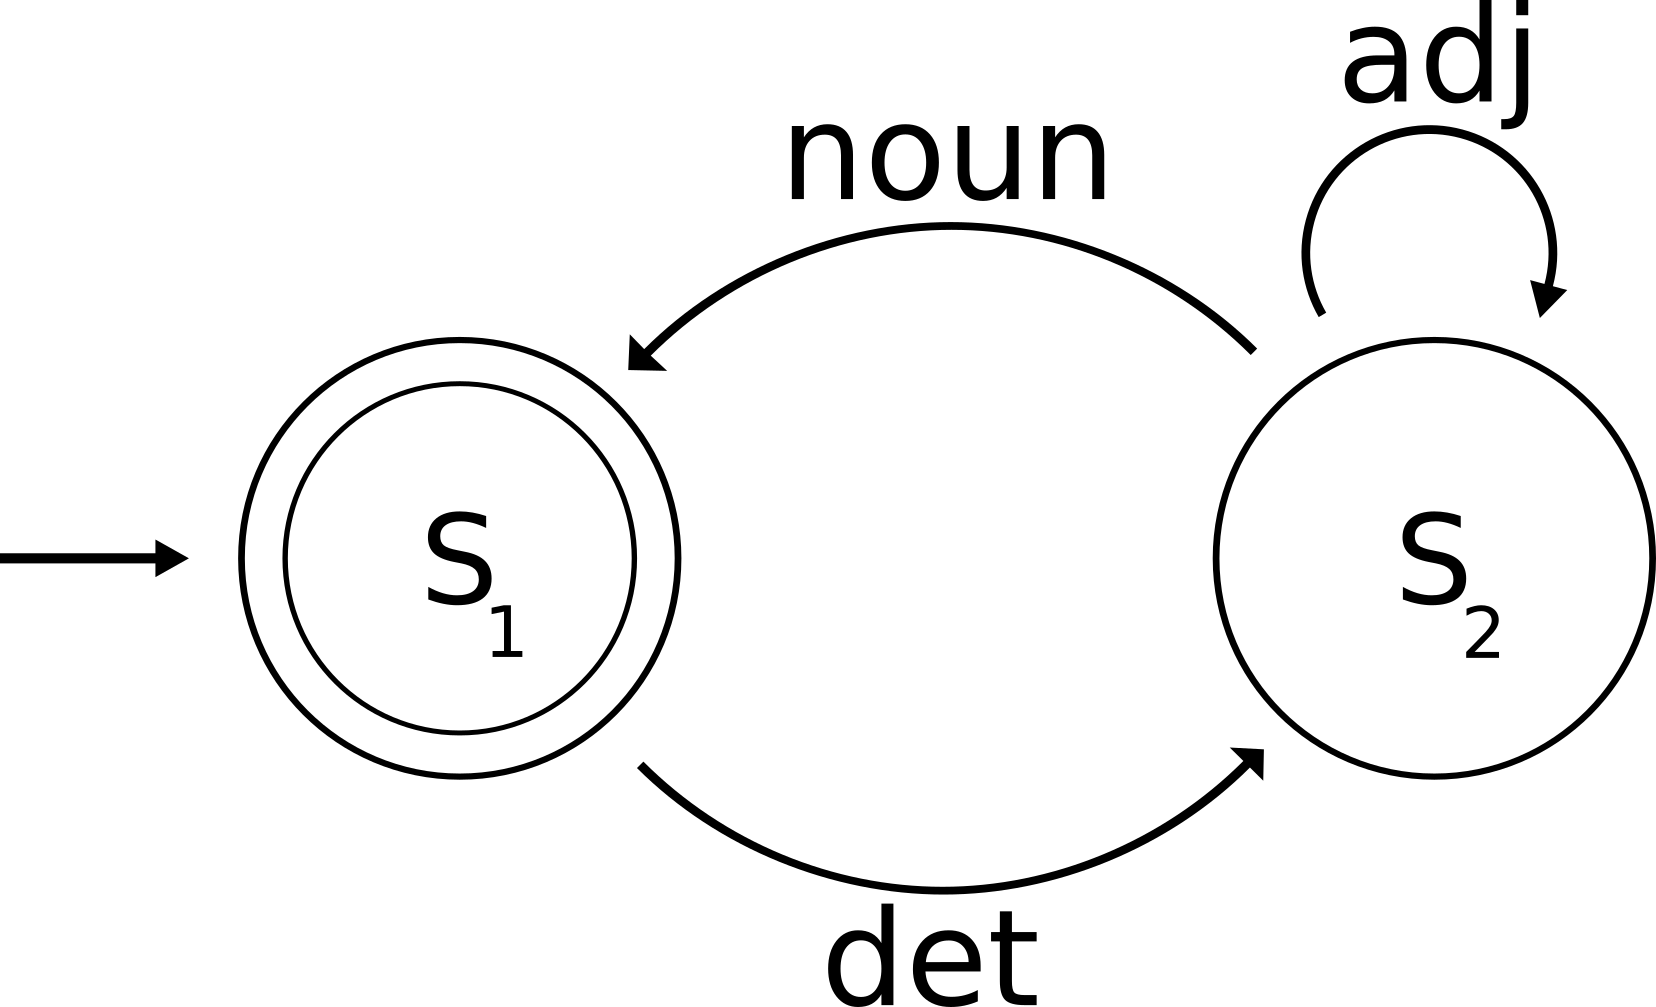
\includegraphics[width=0.4\textwidth]{fsa.png}
  \caption{A finite-state automaton describing the regular language \t{det (adj)* noun}.}
 \label{fig:fsa}
\end{figure}


\section{Beyond regular}

We have not found a general method for other classes. 
However, we can write some example grammars that go beyond regular and context-free.

\subsection{CG is beyond regular}

We can express $a^nb^n$, here's the grammar.

\subsection{CG is beyond context-free}

We can express $a^nb^nc^n$, here's the grammar.  

\section{Discussion}

Practical benefits: derive CGs from perhaps more easily defined formalisms?

CG can act as a preprocessing step for some more expensive parser. Then the rules can be non-human-oriented, and contain extra symbols. The rules would be derived from the grammar itself, with the sole purpose of making the parsing \emph{faster}, not more accurate.

% \section*{Acknowledgments}

% Do not number the acknowledgment section. Do not include this section
% when submitting your paper for review.





\bibliographystyle{acl}
\bibliography{cg}


\end{document}
